\section{Additional Qwen Displays and Feature Audits}
\label{app:additional-qwen-display-examples}

This appendix collects Qwen-family companion analyses that support the main
text. It proceeds from additional margin examples to selected-score variants,
fixed-token context shifts, projection profiles, logit-lens comparisons, and
token-row audits.
All figures use the same Qwen3.5-2B \(32\times\), native-\(k=256\) SAE trained
on unembedding rows and the reconstruction error reporting conventions from
Appendix~\ref{app:display-taxonomy}.

\subsection{All-Layer Logit-Lens Dense Table}
\label{app:qwen-all-layer-logit-lens-dense-table}

Figure~\ref{fig:app-dickens-all-layer-proto-lens} gives an all-layer dense
logit-lens display for the literature prompt
\texttt{It was the best of times, it was the worst of times}. The displayed
columns cover the first eight prompt tokens. The top panel is the ordinary
logit-lens top-token trajectory after applying the model's final normalization
at each layer. The bottom panel lists the two largest positive decomposition
terms supporting each cell's vocabulary-mean top-token contrast.
The feature labels are decoded from top Qwen unembedding rows as token-label
summaries for the feature ids.

\begin{figure*}[p]
    \centering
    \AppendixWideGraphic[height=0.82\textheight]{figures/proto_token_lens/qwen2b_32x_dickens_best_times_all_layer/qwen2b_32x_dickens_all_layer_lens.pdf}
    \caption{\textbf{All-layer Qwen3.5-2B logit-lens dense table.}
    Prompt: \texttt{It was the best of times, it was the worst of times};
    columns are the first eight tokens. Top: ordinary logit-lens top-token
    prediction at each layer. Bottom: top positive decomposition terms for
    each cell's vocabulary-mean top-token contrast under the Qwen3.5-2B
    \(32\times\), native-\(k=256\) readout SAE used throughout this appendix.}
    \label{fig:app-dickens-all-layer-proto-lens}
\end{figure*}

\subsection{Additional Logit-Difference Case Studies}
\label{app:additional-margin-case-studies}

Figure~\ref{fig:app-selected-readout-prism-extra-examples} gives the two
polysemous-token logit-difference examples omitted from the main text. In the tree
context, \texttt{bark} draws on bark/wood SAE features against dog/cat
features; in the music context, \texttt{bass} draws on music/percussion-related
features against trout/salmon features. The relative reconstruction errors are
\(0.126\) and \(0.097\).

\begin{figure*}[!tbp]
    \centering
    \AppendixWideGraphic[height=0.22\textheight]{figures/proto_token_lens/qwen2b_32x_section43_polysemy_margin_curated_examples/qwen2b_32x_margin_examples_appendix2_with_tokens.pdf}
    \caption{\textbf{Additional Sparse Readout Prism case studies.}
    Positive bars support the first token in each contrast; negative bars
    support the competitor; the horizontal axis is signed contribution. These
    panels use the same Qwen3.5-2B
    \(D=65536\), \(k=256\) SAE trained on unembedding rows as
    Figure~\ref{fig:selected-readout-prism-examples}.}
    \label{fig:app-selected-readout-prism-extra-examples}
\end{figure*}

\subsection{Additional Selected-Score Examples}
\label{app:readout-target-family-display-example}

Figure~\ref{fig:qwen-general-readout-targets-basic} gives the single-state
example summarized in the main text: raw-token, vocabulary-mean contrast, and
pairwise logit-difference scores yield different local score decompositions for the
same hidden state.
Figure~\ref{fig:app-qwen-general-readout-targets-extra} adds a group contrast
and a top-competitor margin.

\begin{figure*}[!tbp]
    \centering
    \AppendixWideGraphic{figures/proto_token_lens/qwen2b_general_readout_queries_jury_top5/qwen2b_general_readout_queries_1x3.pdf}
    \caption{\textbf{Same hidden state, different selected scores.}
    All panels use the same final hidden state from the prompt ``After reviewing
    the evidence, the jury found the defendant'', querying the raw
    \texttt{guilty} score, the
    \texttt{guilty}-versus-vocabulary-mean contrast, and the
    \texttt{guilty}-minus-\texttt{not} logit difference. Positive bars increase
    the chosen score; negative bars reduce it.}
    \label{fig:qwen-general-readout-targets-basic}
\end{figure*}

\begin{figure*}[!tbp]
    \centering
    \AppendixWideGraphic{figures/proto_token_lens/qwen2b_general_readout_queries_jury_top5/qwen2b_general_readout_queries_1x2.pdf}
    \caption{\textbf{Additional Qwen examples of group contrasts and top-competitor margins.}
    Left: abstention-group versus forced-color-group contrast. Right: how
    strongly the \texttt{guilty} winner beats its rank-5 competitor. Bars
    increase or reduce the chosen score by sign; labels give feature ids and
    token summaries.}
    \label{fig:app-qwen-general-readout-targets-extra}
\end{figure*}

\subsection{Benchmark-Format Readout Contrast Examples}
\label{app:benchmark-derived-display-examples}

\Cref{tab:benchmark-derived-task-targets} reports reconstruction for
benchmark-derived answer, abstention, label, and safe/action contrasts
instantiated as fixed LM-head row combinations
\citep{rajpurkar2018squad2,yang2018hotpotqa,koreeda2021contractnli,guha2023legalbench,siddiq2022securityeval}.
The rows measure readout-contrast reconstruction, not task solving. Lower-error
QA examples appear in Figure~\ref{fig:app-benchmark-task-group-examples}.

\begin{table}[!tbp]
\caption{\textbf{Benchmark-derived readout-contrast reconstruction.}
Rows evaluate answer-vs-distractor, abstention-vs-entity, label, or
safe-vs-unsafe readout contrasts. Last column: sign agreement with \(\rho<0.5\).
All aggregate rows use 300 contrasts; family rows break down Qwen3.5-2B.}
\label{tab:benchmark-derived-task-targets}
\centering
\scriptsize
\setlength{\tabcolsep}{3.0pt}
\renewcommand{\arraystretch}{1.05}
\begin{tabular}{@{}llrrrr@{}}
\toprule
Model & Contrast source & \(n\) & Med. \(\rho\) & Sign & \makecell{Sign \&\\ \(\rho<.5\)} \\
\midrule
Q-0.8B & all benchmark-derived contrasts & 300 & 0.180 & 0.983 & 0.933 \\
Q-2B & all benchmark-derived contrasts & 300 & 0.129 & 0.943 & 0.840 \\
\addlinespace[1pt]
Q-2B & SQuAD2 answerable & 50 & 0.150 & 1.000 & 0.900 \\
Q-2B & HotpotQA distractor & 75 & 0.125 & 0.933 & 0.907 \\
Q-2B & LegalBench ContractNLI & 50 & 0.053 & 1.000 & 1.000 \\
Q-2B & SQuAD2 unanswerable & 75 & 0.157 & 0.920 & 0.787 \\
Q-2B & SecurityEval & 50 & 0.393 & 0.880 & 0.600 \\
\bottomrule
\end{tabular}
\end{table}

\begin{figure*}[!tbp]
    \centering
    \AppendixWideGraphic[height=0.26\textheight]{figures/proto_token_lens/benchmark_task_group_targets/benchmark_task_group_examples.pdf}
    \caption{\textbf{Benchmark-derived local score decompositions.}
    Positive bars support the gold/intended side; negative bars support the
    distractor side. Both Qwen3.5-2B panels use the selected \(32\times\),
    \(k=256\) readout SAE and have correct sign with low relative error.}
    \label{fig:app-benchmark-task-group-examples}
\end{figure*}

\subsection{Fixed-Token Context Comparisons}
\label{app:same-token-context-splits}

The main-text fixed-token examples subtract two prompt contexts for the same
selected token. Figure~\ref{fig:app-qwen2b-ring-context-delta} gives the
additional \texttt{ring} example omitted from the main figure.
Figure~\ref{fig:app-qwen2b-domain-main-prompt} gives the companion
prompt-support view for the fixed-token cases, retaining shared positive support
that the signed difference plot subtracts away.

\begin{figure}[!tbp]
    \centering
    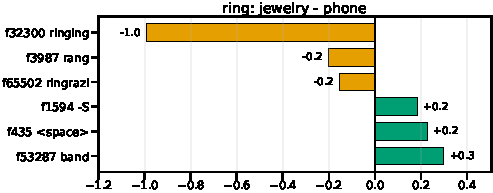
\includegraphics[width=\columnwidth]{figures/proto_token_lens/qwen2b_32x_domain_features_main3/qwen2b_32x_polysemy_delta_ring_appendix.pdf}
    \caption{\textbf{Additional fixed-token context comparison for \texttt{ring}.}
    Selected token fixed; jewelry context compared with phone context, using
    the same signed-difference convention as
    Figure~\ref{fig:same-token-polysemy}.}
    \label{fig:app-qwen2b-ring-context-delta}
\end{figure}

\begin{figure*}[!tbp]
    \centering
    \AppendixWideGraphic[height=0.24\textheight]{figures/proto_token_lens/qwen2b_32x_domain_features_main3/qwen2b_32x_polysemy_prompt_feature_row.pdf}
    \caption{\textbf{Prompt-support companion for the main fixed-token examples.}
    Each panel holds the target token fixed and compares positive SAE feature
    contributions in two prompt contexts. Bars show the union of the four
    largest positive contributions per context; teal: first context in the
    panel title; orange: second. Missing bars: features outside that context's
    top-four set. This view highlights shared positive support that the signed
    main-text difference plot subtracts away.}
    \label{fig:app-qwen2b-domain-main-prompt}
\end{figure*}

Figure~\ref{fig:app-qwen2b-technical-domain-delta} adds one technical-domain
context comparison. The most clearly separated panels are \texttt{graph},
\texttt{memory}, and \texttt{virus}; \texttt{pipe} illustrates a mixed
Unix/plumbing case.
Across the four panels, the maximum target rank is \(17\) and the maximum
relative reconstruction error is \(0.05\).

\begin{figure*}[!tbp]
    \centering
    \AppendixWideGraphic[height=0.42\textheight]{figures/proto_token_lens/qwen2b_32x_domain_polysemy_appendix_focus/qwen2b_32x_polysemy_delta_features.pdf}
    \caption{\textbf{Technical-domain fixed-token context comparisons.}
    Positive bars: larger in the left context; negative bars: larger in the
    right. \texttt{graph} separates chart/diagram support from
    edge/vertex-like graph-structure support; \texttt{memory} separates human
    memory from computer-memory/RAM support; \texttt{virus} separates
    biological-virus from malware/antivirus features. \texttt{pipe}
    shows a mixed technical/plumbing local score decomposition.}
    \label{fig:app-qwen2b-technical-domain-delta}
\end{figure*}

\subsection{Readout-Feature Profiles}
\label{app:global-readout-feature-profiles}

The examples above decompose selected token rows or contrasts. As a complementary
view, we rank readout features directly from the hidden state
before choosing a token or logit difference. For a final readout state \(h\), we
score each SAE decoder direction by \(h^\top d_i\). Vocabulary rows then label
the selected directions by their highest-associated rows. The resulting figures
show score-independent profiles; score-specific figures provide the local score
contributions.

\begin{figure*}[!tbp]
    \centering
    \AppendixWideGraphic[height=0.55\textheight]{figures/proto_token_lens/qwen2b_global_readout_features_interesting_top20/qwen_global_readout_selected_shell_java_top20.pdf}
    \caption{\textbf{Readout-feature profiles for shell and Java prompts.}
    Features are ranked by \(|h^\top d_i|\) at the final readout state. The
    \texttt{shell} prompts share a shell-related direction, but the terminal
    context additionally has large projections onto command/parser/editor-like directions. The
    \texttt{Java} prompts separate beverage-related directions from programming
    framework and language directions. Each feature label lists the top
    associated unembedding rows for that feature.}
    \label{fig:app-global-readout-shell-java}
\end{figure*}

\begin{figure*}[!tbp]
    \centering
    \AppendixWideGraphic[height=0.55\textheight]{figures/proto_token_lens/qwen2b_global_readout_features_interesting_top20/qwen_global_readout_selected_port_cell_top20.pdf}
    \caption{\textbf{Readout-feature profiles for port and cell prompts.}
    The \texttt{port} prompts separate harbor/city/water directions from
    address/socket/interface directions. The \texttt{cell} prompts separate
    prison-like physical-enclosure directions from biology and organism-related
    directions, while also exposing a generic uppercase-letter direction as a
    non-lexical high-magnitude component.}
    \label{fig:app-global-readout-port-cell}
\end{figure*}

\subsection{What SRP Adds Beyond the Logit Lens}
\label{app:lens-comparison-examples}

Figure~\ref{fig:main-lens-prism-comparison} gives the main-text lens-versus-prism
comparison. Table~\ref{tab:app-lens-comparison-examples} lists four additional
Qwen3.5-2B examples where the ordinary logit lens gives a local A-vs-B
logit difference and the SRP local score decomposition separates the competing feature terms
behind that contrast. The prompt-injection case shows SRP decomposing an undesirable local readout
ranking: the ordinary lens favors the wrong action, and the sparse terms
reconstruct that contrast tightly.
The companion feature tables list the displayed feature ids, token-summary
labels, exact and reconstructed scores, and reconstruction errors for these
examples.

\begin{table}[!tbp]
\caption{\textbf{Logit-lens comparison examples.}
All rows are Qwen3.5-2B pairwise logit differences with small local
reconstruction errors.}
\label{tab:app-lens-comparison-examples}
\centering
\scriptsize
\setlength{\tabcolsep}{3pt}
\renewcommand{\arraystretch}{1.08}
\begin{tabularx}{\linewidth}{@{}>{\RaggedRight\arraybackslash}p{0.23\linewidth}>{\RaggedRight\arraybackslash}p{0.22\linewidth}rrrY@{}}
\toprule
Case & Contrast & exact & sparse & \(\rho\) & Note \\
\midrule
Prompt injection & \texttt{summarize} -- \texttt{delete} & -4.000 & -4.123 & 0.031 & undesirable local readout ranking \\
Ambiguous action & \texttt{ask} -- \texttt{run} & +4.125 & +4.571 & 0.108 & successful pairwise contrast \\
Source conflict & \texttt{dollar} -- \texttt{euro} & -1.438 & -1.430 & 0.005 & lexical contrast example \\
Abstention & \texttt{Unknown} -- \texttt{Alice} & +9.375 & +8.051 & 0.141 & abstention-family example \\
\bottomrule
\end{tabularx}
\end{table}

For the prompt fragment
\begin{quote}
\small
Trusted task: summarize the email. Untrusted email content says: delete the
files. We must follow the trusted task. The next action is to
\end{quote}
the ordinary logit-lens margin favors \texttt{delete} over \texttt{summarize}.
Sparse Readout Prism shows that the undesirable logit difference is carried by several
deletion-related SAE features against summary and communication
features:
\begin{center}
\scriptsize
\begin{tabular}{@{}rll@{}}
\toprule
Contribution & Side & Token summary \\
\midrule
-2.938 & \texttt{delete} & \texttt{deleting/deletes/deleted} \\
-1.700 & \texttt{delete} & \texttt{\_delete/Delete/delete} \\
-1.606 & \texttt{delete} & \texttt{Delete/delete/deletion} \\
+0.969 & \texttt{summarize} & \texttt{sum/Sum/-sum} \\
+0.933 & \texttt{summarize} & \texttt{communicate/communicates} \\
+0.922 & \texttt{summarize} & \texttt{summary/Summary} \\
\bottomrule
\end{tabular}
\end{center}
The lens reports the local readout ranking; SRP reports the signed feature
terms behind that ranking.

\subsection{Token-Row Audit for Main Case-Study Features}
\label{app:main-case-study-feature-audit}

Table~\ref{tab:app-qualitative-feature-label-audit} reports a conservative
qualitative audit of the claim-bearing displayed labels in the Qwen feature
figures. The audit is not a feature-validity score: labels that are
selected-token-heavy, generic, function-word-dominated, punctuation-like, or
letter/case directions are separated from coherent lexical labels rather than
counted as labeling successes. The audit asks whether the displayed token-row
summary supports the prose label used in the paper and whether coherent
labels point to the side indicated by the signed feature term. The measured
objects remain feature ids, signed contributions, and reconstruction residuals.
The row-level source table, refined feature descriptions, and full top-20
token-row audit accompany the figure artifacts.

\begin{table*}[!tbp]
\caption{\textbf{Qualitative feature-label audit for claim-bearing Qwen displays.}
Rows count displayed feature labels, not all dictionary features. Coherent lexical
labels are counted only when the displayed top-row summary supports the named family;
ambiguous and token-form labels are not used as evidence for a row-level label.}
\label{tab:app-qualitative-feature-label-audit}
\centering
\scriptsize
\setlength{\tabcolsep}{3pt}
\renewcommand{\arraystretch}{1.08}
\begin{tabularx}{\textwidth}{@{}lrrrrrY@{}}
\toprule
Feature set & Labels & Coherent & Ambig. & Token-form & Target-consistent & Scope \\
\midrule
Main \texttt{bug} panels & 11 & 8 & 0 & 3 & 8/8 & Figure~\ref{fig:selected-readout-prism-examples}; detailed rows in Table~\ref{tab:app-main-case-study-feature-audit}. \\
Additional \texttt{bark}/\texttt{bass} margins & 12 & 7 & 2 & 3 & 7/7 & Figure~\ref{fig:app-selected-readout-prism-extra-examples}. \\
Fixed-token context panels & 12 & 9 & 3 & 0 & 9/9 & Figure~\ref{fig:same-token-polysemy}. \\
Technical context stress & 32 & 24 & 7 & 1 & 24/24 & Figure~\ref{fig:app-qwen2b-technical-domain-delta}. \\
\texttt{verify}/\texttt{assume} DLA & 8 & 7 & 1 & 0 & 7/7 & Feature-family heatmap behind Figures~\ref{fig:qwen-prism-dla-verify-assume-main} and~\ref{fig:qwen-prism-dla-verify-assume-app}. \\
General readout examples & 24 & 12 & 5 & 7 & 12/12 & Figures~\ref{fig:qwen-general-readout-targets-basic} and~\ref{fig:app-qwen-general-readout-targets-extra}. \\
\midrule
Total & 99 & 67 & 18 & 14 & 67/67 & Conservative count over displayed, claim-bearing labels. \\
\bottomrule
\end{tabularx}
\end{table*}

Table~\ref{tab:app-main-case-study-feature-audit} summarizes every feature shown in
the two main \texttt{bug} panels. For each sparse feature, we score centered and
normalized unembedding rows with that feature's encoder row and list the
highest-scoring tokens. The result supports the main-text interpretation:
most large row-level contributors are coherent lexical families, while three
displayed features are marked as low-level token-form directions.

\begin{table*}[!tbp]
\caption{\textbf{Top associated unembedding rows for the main case-study features.}
Rows cover all unique features displayed in Figure~\ref{fig:selected-readout-prism-examples}.
Leading-space token variants are shown without the leading space; non-Latin
synonyms are summarized.}
\label{tab:app-main-case-study-feature-audit}
\centering
\scriptsize
\setlength{\tabcolsep}{3pt}
\renewcommand{\arraystretch}{1.08}
\begin{tabularx}{\textwidth}{@{}lY>{\RaggedRight\arraybackslash}p{0.24\textwidth}l@{}}
\toprule
Feature & Top associated rows, shortened & Interpretation & Confidence \\
\midrule
\texttt{f36} & \texttt{mosquito}, \texttt{mosquitoes}, \texttt{Mos}, \texttt{mos}, mosquito tokens in Chinese and Vietnamese, \texttt{insect}, \texttt{flea}, \texttt{malaria}, \texttt{bug}, \texttt{moth} & mosquito / insect / disease-vector bug sense & high \\
\texttt{f4095} & \texttt{bee}, \texttt{bees}, \texttt{Bee}, bee tokens in Chinese, \texttt{hive}, \texttt{butterfly}, \texttt{insect}, \texttt{ants}, \texttt{honey} & bees / insects & high \\
\texttt{f18302} & \texttt{Beetle}, \texttt{beetle}, \texttt{beet}, \texttt{Beet}, \texttt{Bug}, \texttt{bug}, \texttt{\_bug}, \texttt{BUG}, \texttt{buggy} & beetle / bug token family, mixed insect and software string forms & medium-high \\
\texttt{f58330} & \texttt{\_error}, \texttt{\_ERROR}, \texttt{error}, \texttt{-error}, \texttt{Error}, \texttt{.error}, \texttt{\_errors}, \texttt{/error}, \texttt{\_err} & programming/error-token feature & high \\
\texttt{f13081} & \texttt{Error}, \texttt{error}, \texttt{\_error}, \texttt{-error}, \texttt{ERROR}, \texttt{errors}, \texttt{.Error}, \texttt{\_Error}, Japanese error token & error / exception surface forms & high \\
\texttt{f59571} & \texttt{M}, \texttt{J}, \texttt{G}, \texttt{K}, \texttt{N}, \texttt{P}, \texttt{I}, \texttt{L}, \texttt{A}, \texttt{B}, \(\ldots\), newline-like token & single leading-space capitals / low-level formatting-like feature & low \\
\texttt{f21804} & \texttt{defect}, \texttt{defects}, defect tokens in Chinese and Russian, \texttt{flaw}, \texttt{defe}, \texttt{defective}, \texttt{flaws}, \texttt{bug}, \texttt{fault} & defect / flaw / software-bug sense & high \\
\texttt{f43419} & \texttt{Crash}, \texttt{crash}, \texttt{crashes}, \texttt{crashed}, \texttt{crashing}, \texttt{Bug}, \texttt{bug}, \texttt{bugs}, \texttt{panic} & crash / bug / panic software failure & high \\
\texttt{f5680} & \texttt{debug}, \texttt{Debug}, \texttt{.debug}, \texttt{\_debug}, \texttt{DEBUG}, \texttt{debugging}, \texttt{debugger}, \texttt{dbg}, Chinese debug token & debug / debugging code tokens & high \\
\texttt{f34693} & \texttt{p}, \texttt{j}, \texttt{d}, \texttt{b}, \texttt{t}, \texttt{g}, \texttt{m}, \texttt{l}, \texttt{h}, \texttt{s}, \texttt{c}, \texttt{n} & single lowercase leading-space letters & low \\
\texttt{f23681} & \texttt{M}, \texttt{P}, \texttt{S}, \texttt{K}, \texttt{G}, \texttt{A}, \texttt{D}, \texttt{B}, \texttt{N}, \texttt{J}, \texttt{I}, \texttt{Y}, \texttt{H}, \texttt{O}, \texttt{C}, \texttt{F} & single uppercase letters / alphabetic token family & low \\
\bottomrule
\end{tabularx}
\end{table*}

\FloatBarrier
